\chapter{Gluon saturation}
\label{chp:saturation}

The idea of saturation physics can be briefly described as follows: when the
gluon density at low $x$ becomes so large that different gluon clouds with fixed
transverse size $\sim 1/Q^{2}$ start to overlap with each other, the QCD
evolution dynamics essentially becomes nonlinear~\cite{Gribov:1984tu,Mueller:1985wy}. 
It is conceivable that gluons which occupy the same area $\sim 1/Q^{2}$ can recombine with a cross section $\sigma_{gg\rightarrow g}\simeq \alpha_{s}/Q^{2}$, thereby taming further
rapid growth of the gluon density (as shown in Fig.~\ref{fig:recombine}). This nonlinear evolution can be encoded by the extension of the BFKL
equation as the Balitsky-Kovchegov (BK) equation~\cite{Balitsky:1995ub}.
\begin{figure}
\centering
\includegraphics[width=0.8\textwidth]{plots/chpt3/recomb.pdf}
\caption[A schematic view of parton recombination process]{
A schematic view of the parton recombination process. This plot is from Ref.~\cite{Accardi:2012qut}.}
\label{fig:recombine}
\end{figure}

This non-linear dynamical effect can be enhanced with a nuclear target, where the
interaction develops over a longitudinal distance of the order of the nuclear size
or larger. 
In this case the nucleons located at the same impact factor
cannot be distinguished from each other. Gluons from different nucleons can
amplify the total transverse gluon density by a factor of $A^{1/3}$ for a
nucleus with mass number $A$. 

\section{Saturation scale}

\begin{figure}
\centering
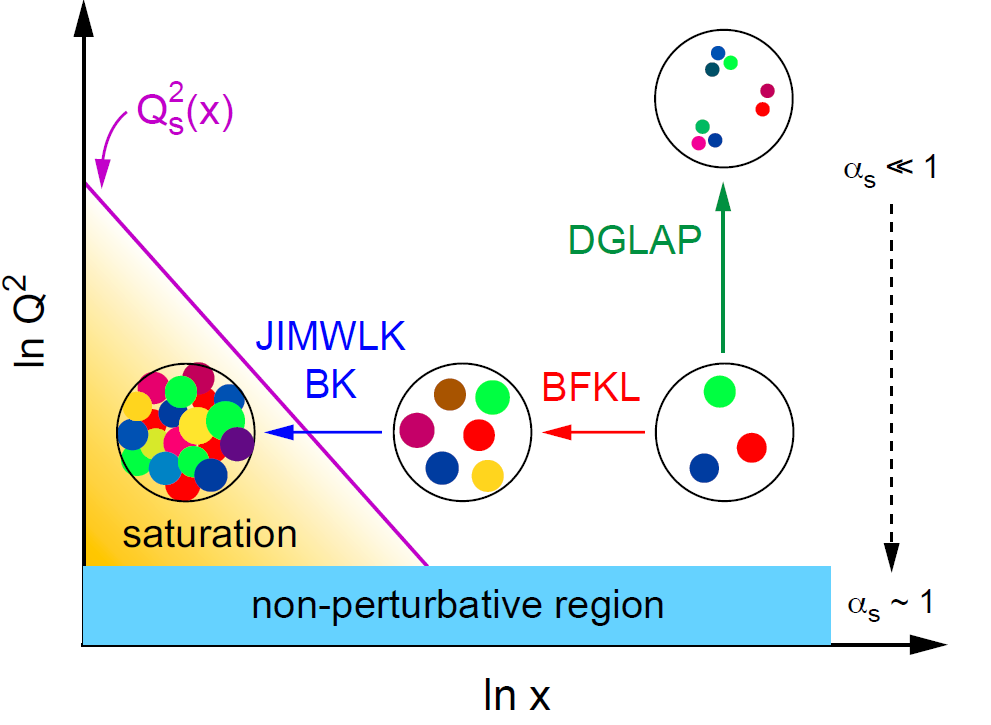
\includegraphics[width=0.65\textwidth]{plots/chpt3/Q2Vx_map.png}
\caption[Evolution approaches in $Q^{2}$ vs $x$ plane]{
Map of high energy QCD in the $Q^{2}$ and $x$ plane. This plot is from Ref.~\cite{Accardi:2012qut}.}
\label{fig:Q2vX_map}
\end{figure}

To get a crude quantitative feel about the magnitude of saturation scale, 
we define a gluon-gluon recombination or absorption cross section \(\sigma_{gg}\sim\alpha_{s}(Q^{2})/Q^{2}\).
In the infinite momentum frame, $N_{g}\sim xg(x,Q^{2})$ gives the number of gluons per unit of $dx/x$.
Thus, one may expect the saturation effects arise when the total effective gluon-gluon recombination
cross section in the proton approaches the size of the proton disk as
\[\sigma_{gg} \cdot N_{g}|_{Q=Q_{s}} \sim \pi R^{2},  \]
in which $R$ corresponds to the proton radius. On the ground of that,
a saturation scale can be estimated as $Q^{2}_{s}\sim \alpha_{s}\frac{xg(x,Q^{2}_{s})}{\pi R^{2}}\sim x^{-\lambda}$.

Typically, a characteristic scale $Q_{s}(x,A)$ can
be introduced to describe the transition to the saturation region. 
\begin{equation}
Q^{2}_{s}(x,A)\simeq A^{1/3} Q^{2}_{0}(\frac{x}{x_{0}})^{-\lambda},
\label{eqn:sat_scale}
\end{equation}
with $\lambda$ known as the saturation exponent. $Q^{2}_{0}$ is the proton
saturation scale at the original value $x_{0}$. These parameters are
non-perturbative and can only be fitted from the data. 
For a large nucleus, the incoming projectile sees the gluons from different nucleons coherently in the longitudinal direction. Note that the transverse gluon occupation number is likely to be enhanced in nuclei by a factor of $A^{1/3}$.
%The generation of the transverse momentum for the scattered projectile on a
%large nucleus can be interpreted as follows: the incoming probe acquires
%transverse momentum kicks from all the nucleons the at the same impact
%parameter. Similar to a random walk process, after $A^{1/3}$ kicks the typical
%transverse momentum generation from a nucleus (or the saturation scale for a
%nucleus target) 
The saturation scale for a nucleus target becomes larger than that for a proton varying as
$Q_{sA}^{2}\approx A^{1/3}Q^{2}_{sp}$. This enhancement factor $A^{1/3}$ due to
the existence of the nuclear environment is often referred to as the nuclear
``oomph" factor.

For $Q^{2}>Q_{s}^{2}$, the target hadron and nucleus is usually treated as a dilute system,
whereas $Q^{2}<Q_{s}^{2}$ corresponds to the case with a highly saturated
hadron with a large parton density. Therefore, as seen in
Fig.~\ref{fig:Q2vX_map}, one can define a boundary with $Q^2=Q_s^2(x)$ in the
$x\textrm{-}Q^2$ plane to describe the transition from the non-linear saturation
regime to the linear dilute regime. The main physical ingredient of the
saturation formalism is to incorporate the unitarity constraint for high-energy
scattering amplitudes through the inclusion of non-linear recombination in the
quantum evolution of hadronic wave functions.


\section{Color glass condensate}\label{sec:CGC}
The partonic form of the matter made with the saturated gluons can be described in the color glass condensate framework (CGC)~\cite{Iancu:2002xk}. The saturation momentum scale
increases with $1/x$. For sufficiently small $x$, $Q^{2}_{s}>>\Lambda_{QCD}$ and
hence $\alpha_{s}(Q^{2}_{s})<<1$, the CGC is weakly coupled and we should be
able to perform a perturbative calculation. Based on that, our strategy will be
to construct an effective theory, which resums an infinite series of the large
logarithms enhanced by the small $x$. The key ingredient in this scenario is to
describe the small-$x$ gluons as the classical color fields radiated by the fast
partons (valence quarks) with large $x$. Generally, fast partons are seen as the
color source for the classical color fields. The kinematical distinction makes
the foundation for the Mclerran-Venugopalan (MV) model~\cite{McLerran:1993ni}.
With this distinction, we can calculate the non-linear effects exactly within
the classical context.

According to the MV model, the dominant gluon field is given by the solution of
the classical Yang-Mills equations~\cite{Kovchegov:1996ty}, with
which one can construct an unintegrated gluon distribution $\mathcal{F}(x,k^{2}_{T})$
shown in Fig.~\ref{fig:gluon_TMD}. The majority of the gluons have transverse
momenta $k_{T}\approx Q_{s}$. Unlike the prediction of linear perturbative
theory for the gluon distribution at $k_{T}\sim0$, the growth of gluon distribution
for $k_{T}<Q_{s}$ is largely suppressed or saturated as the name suggests.
\begin{figure}
\centering
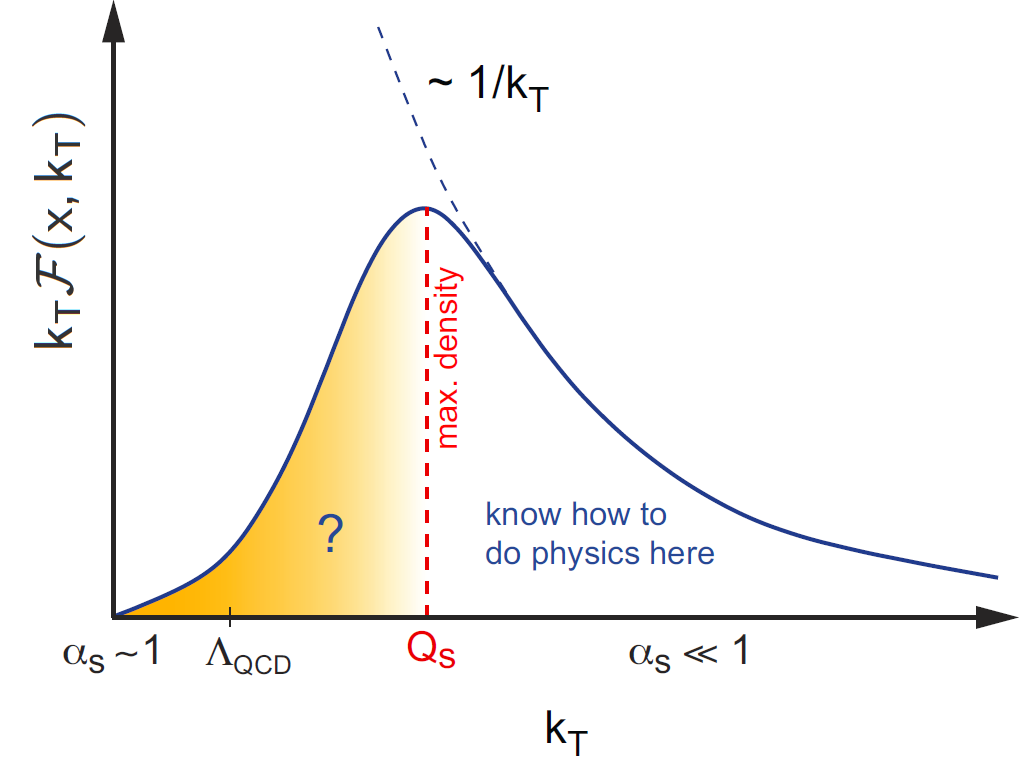
\includegraphics[width=0.65\textwidth]{plots/chpt3/kt_schematic.png}
\caption[Unintegrated gluon transverse momentum distribution]{
The unintegrated gluon distribution of a large nucleus from CGC (solid). The dashed curve 
shows the perturbative result with linear evolution. This plot is from Ref.~\cite{Accardi:2012qut}.}
\label{fig:gluon_TMD}
\end{figure}


%
%\subsection{Geometric scaling}
%Geometric scaling is a striking feature of the experimental data observed at
%HERA with $x_{Bj}<0.01$~\cite{Stasto:2000er}, shown by
%Fig.~\ref{fig:geo_scaling}. Generally, one would expect the virtual photon
%proton cross section depends on two kinematics variables $Q^{2}$ and $x_{Bj}$
%independently. However, Measurements at HERA showed that the virtual photon
%proton cross section scales with a single variable $\tau=Q^{2}/Q^{2}_{s}$, in
%which $Q_{s}$ is the saturation scale. Such a scaling behavior has been
%consistently described in the saturation scenario~\cite{GolecBiernat:1998js}. On
%the other hand, the experimentally observed scaling also extends to the kinematics
%region out of the estimated saturation regime. Hence, this scaling feature seems
%to be more general than the saturation and more detailed comparisons with data
%are necessary.
%\begin{figure}
%\centering
%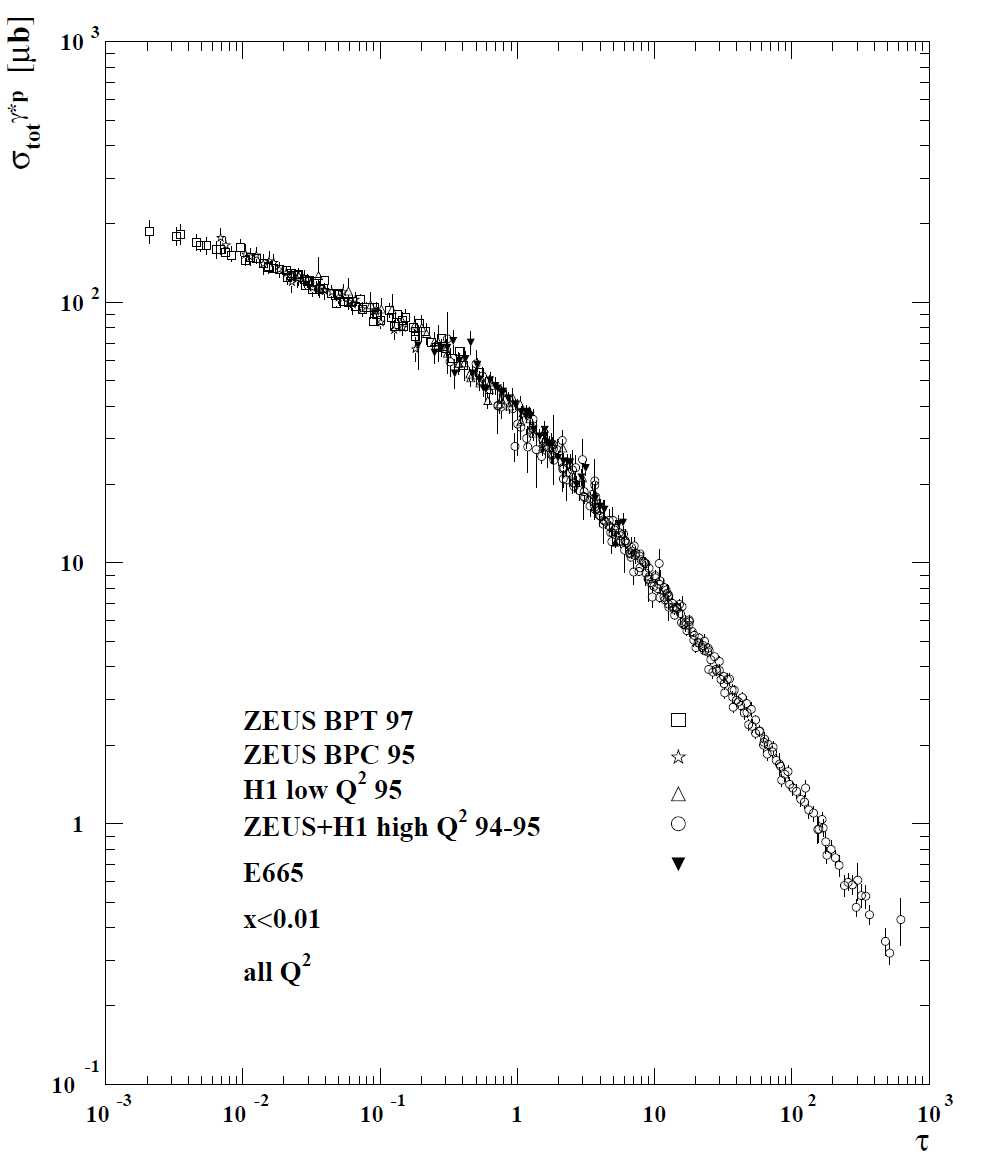
\includegraphics[width=0.7\textwidth]{plots/chpt3/geo_scaling.png}
%\caption[Geometric scaling]{
%Geometric scaling of $\gamma^{*}p$ cross section varying with a single scaling variable
%$\tau=Q^{2}/Q^{2}_{s}$. This plot is from Ref.~\cite{Stasto:2000er}.}
%\label{fig:geo_scaling}
%\end{figure}
%
%\subsection{Nuclear modification factor}
%
%Nuclear modification factor is an observable that has magnetized much of the
%discussion on the saturation physics in $d+$Au collisions at RHIC. In this observable, the nuclear effects can be evaluated in terms of
%the ratio of inclusive particle yields from \dA\ and $p+p$ collisions
%\begin{equation} R_{dAu}=\frac{dN^{dAu\rightarrow
%hX}/dydp_{T}}{N_{coll}dN^{pp\rightarrow hX}/dydp_{T}}. 
%\end{equation} 
%$N_{coll}$ is the number of binary nucleon-nucleon collisions in one \dA\
%collision. If \dA\ collisions were incoherent superpositions of elementary
%nucleon-nucleon collision, the value should be around unity. On the basis of the
%saturation theory, a homogeneous suppression is expected moving from the mid-rapidity
%region to forward rapidities~\cite{Albacete:2014fwa}. It is assumed that in the
%$d+$Au, there's no large final-state effect. Therefore,
%this signature is a clear indication of nuclear effects in the initial state.
%This expectation is observed in the data (see Fig.~\ref{fig:fwd_single_dAu}) and
%a good quantitative description is achieved within the CGC.
%\begin{figure}
%\centering
%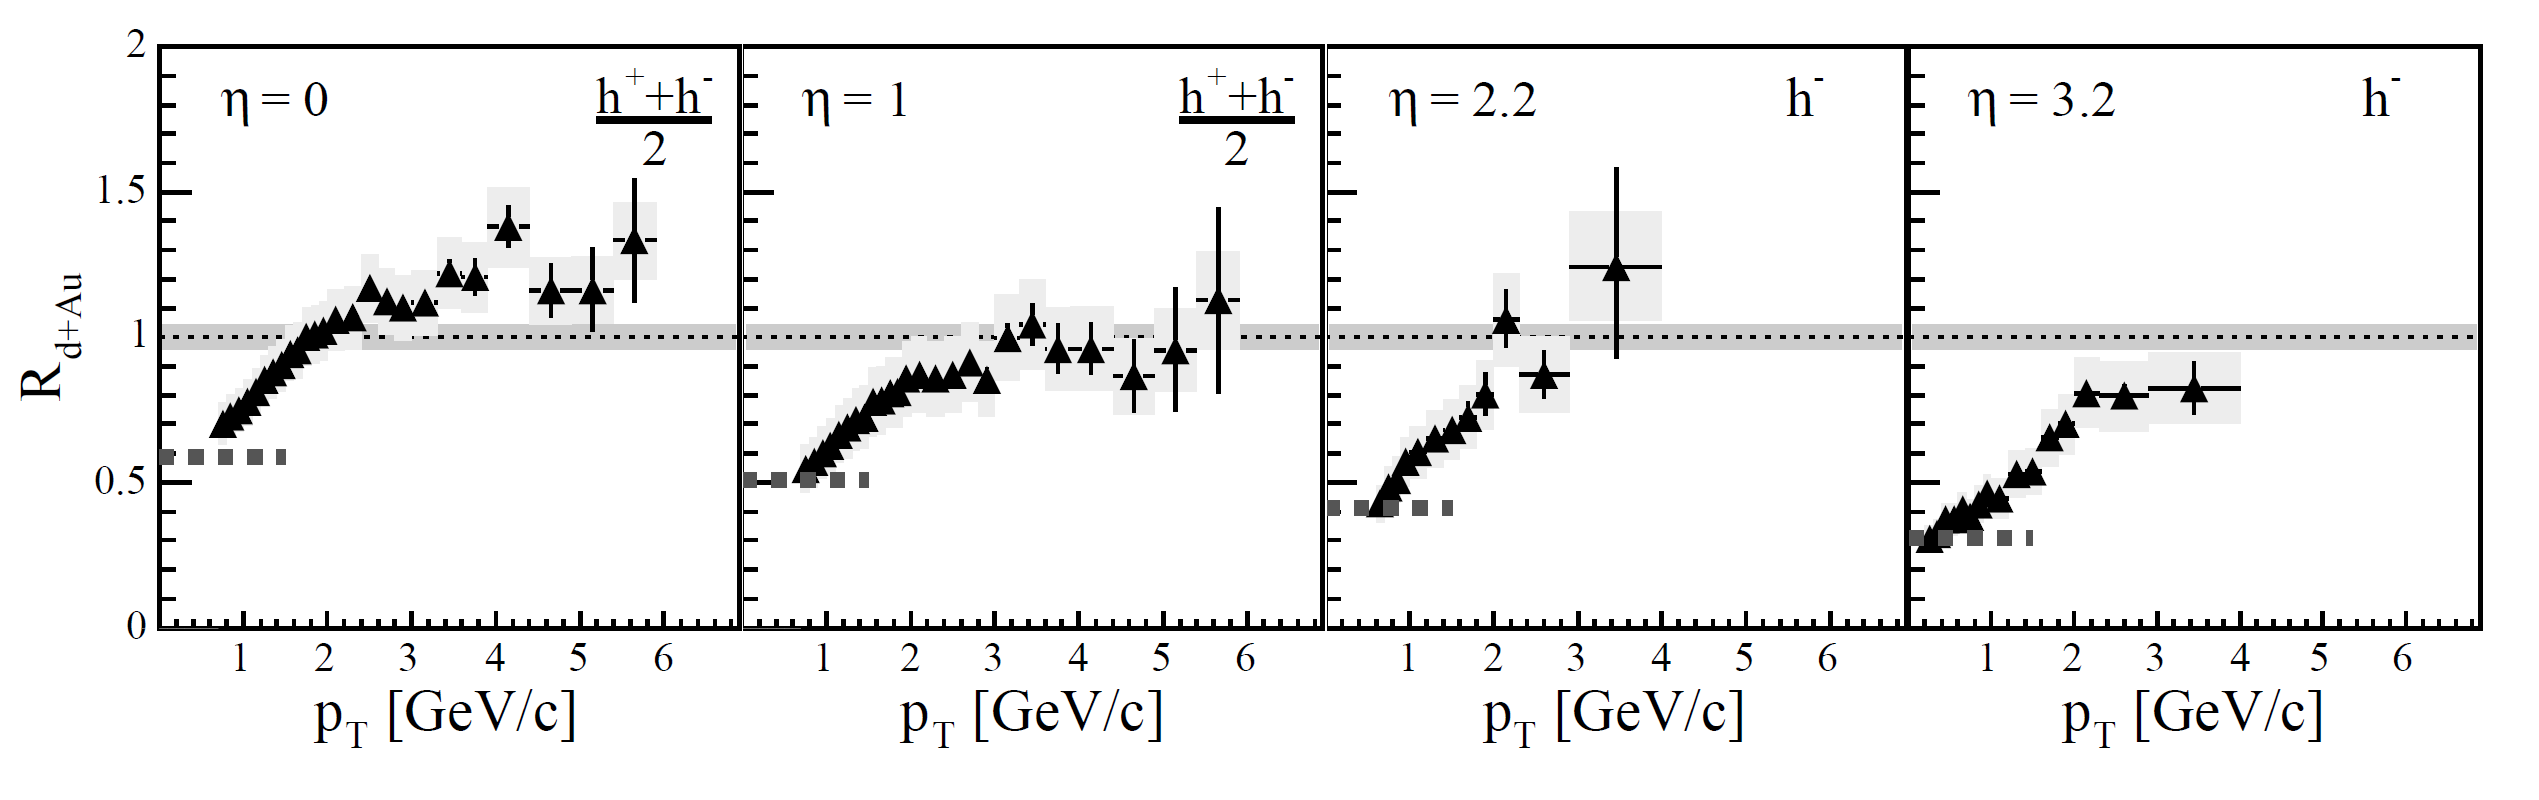
\includegraphics[width=1.0\textwidth]{plots/chpt3/fwd_single_dAu.png}
%\caption[Nuclear modification factors in $d+$Au]{
%Nuclear modification factors from mid-rapidity to forward rapidity region in \dA\ collisions at RHIC. This plot is from Ref.~\cite{Arsene:2004ux}.}
%\label{fig:fwd_single_dAu}
%\end{figure}
%However, other than the CGC approaches, alternative formalisms also reproduce
%the data successfully~\cite{Kopeliovich:2005ym}. It has been argued that large-$x$
%effects such as energy loss neglected in the CGC approach may also be relevant.
%Thus, it is difficult to extract any clean conclusion about the physical origin
%of the forward suppressions. Different physical mechanisms concur and further studies
%are needed.
%


\section{Saturation studies to be performed at an EIC} \label{sec:eic_eA_physics}

It is a challenging task to determine to what extent saturation is present at
currently running high-energy experimental facilities~\cite{Albacete:2010rh}. In
the saturation regime, the interaction is described by the coherent scattering
of the probe from multiple partons collectively correlated in a high density
medium following the CGC picture. To achieve an accurate description of
experimental data, it is essential to have theoretical calculations beyond
the leading order, especially as the higher-order corrections are known to be
sizable. Practically, phenomenological models have been applied to describe a
wide range of experimental data with a few input parameters.

One of the major targets of the \eA\ program at an EIC is to unveil the
collective behavior of densely packed gluons in the saturation regime. As we
argued above, the saturation scale grows with decreasing $x$ and with the
increasing mass number of a nucleus $A$. Collisions with nuclei probe the
saturation region at significantly larger $x$ than would be possible in \ep\
collisions. While at an EIC, it is impossible to directly study the behavior of
saturated gluons in the proton, the $A^{1/3}$ enhancement factor allows us to
perform the saturation studies with large nuclei. We will learn from the
thorough comparison of investigating a multitude of measurements performed on
different ion species. A wide range of measurements with an EIC can distinguish
between predictions from novel theory frameworks like CGC and linear QCD
evolutions established on DGLAP equations.

Compared to the \dA\ program at RHIC, there are several advantages of performing
the saturation studies at an EIC. The predictive power of CGC strongly depends
on the amount of non-perturbative inputs (e.g. initial conditions for small $x$
evolution, impact parameter dependence) needed for the calculations. \eA\
collisions undoubtedly provide the best option to decrease these uncertainties
as much as possible. In addition, with kinematics variables determined event by
event, one can pin down the underlying gluon dynamics more precisely compared to
\dA\ collisions. We will illustrate some key measurements related to the
search of saturation physics at an EIC.

\subsection{Longitudinal structure function}
The total DIS cross section is related to structure functions $F_2$ and $F_L$ by
a linear relation. In the naive quark parton model, transverse momentum of the
partons is assumed to be zero and accordingly we have $F_{L}=0$. The QCD
inspired higher order corrections give rise to partons with non-negligible
transverse momentum and $F_{L}$ becomes nonzero starting from
$\mathcal{O}(\alpha_{s})$ receiving contributions from both quarks and gluons as
shown in Eq.~\ref{eqn:FL}:
\begin{equation}
\frac{F_{L}(x_{Bj},Q^{2})}{x_{Bj}}=\frac{\alpha_{s}}{2\pi}\int^{1}_{x_{Bj}}\frac{d\xi}{\xi}[\sum_{i}e^{2}_{i}\frac{8}{3}(\frac{x_{Bj}}{\xi})q_{i}(\xi,Q^{2})
+{\bar{e}}^{2}4(\frac{x_{Bj}}{\xi})(1-\frac{x_{Bj}}{\xi})g(\xi,Q^{2})], \label{eqn:FL}
\end{equation}
in which $\bar{e}^{2}=\sum_{i}e_{i}^{2}$. $\xi$ shows the momentum fraction of the parton involved in the hard interaction, $q(\xi,Q^{2})$ and
$g(\xi,Q^{2})$ represent the quark and gluon distribution respectively. 
At low $x$, the gluon contribution greatly exceeds the quark contribution. Therefore, measuring $F_{L}$ provides a rather direct
way to study the underlying gluon dynamics with high parton density.

As saturation is mainly driven by the gluon dynamics, we are expected to see
stronger signals in $F_L$. The nuclear effects on the longitudinal structure
function can be quantified as follows:
\begin{equation}
R_{L}(x_{Bj},Q^{2})=\frac{F^{A}_{L}(x_{Bj},Q^{2})}{AF^{p}_{L}(x_{Bj},Q^{2})}.
\end{equation}
In the absence of any nuclear effects, $R_L$ should be unity. 

In Fig.~\ref{fig:F_L}, two calculations for $F_L$ are presented. The blue one is
obtained within the CGC framework~\cite{Albacete:2009fh}, while the gray band uses the
NLO DGLAP evolution based on the EPS09 nuclear PDF. For heavy ions $R_L$ shows a
significant suppression due to the existence of the nuclear environment,
while this ratio becomes unity at $A\sim 1$. 
\begin{figure}
\centering
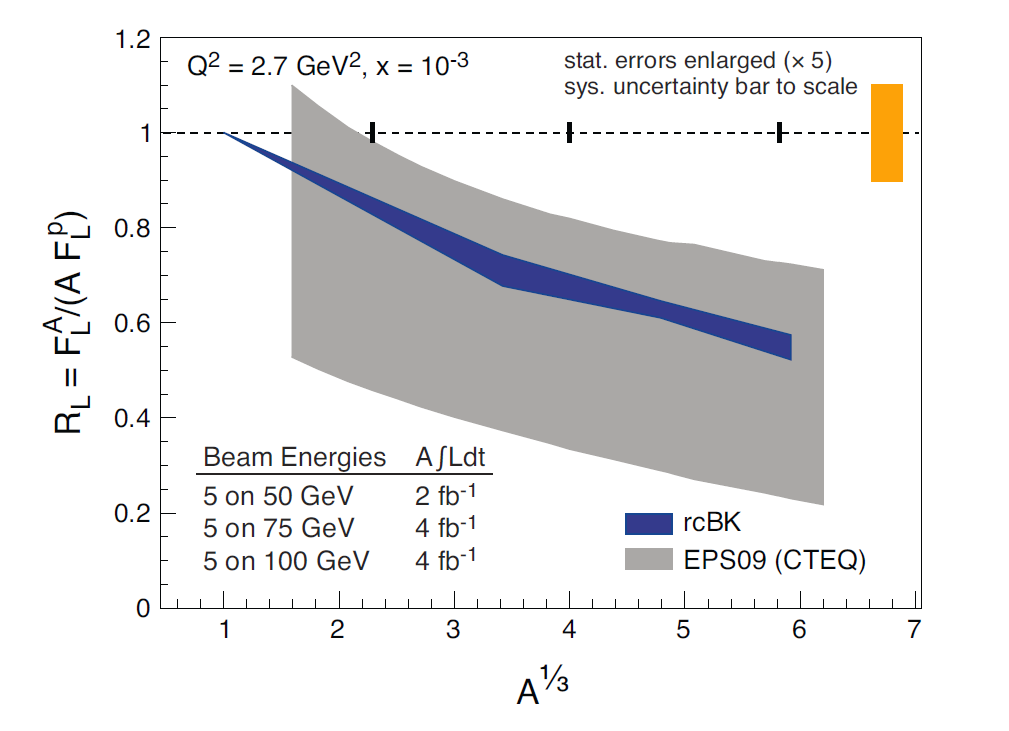
\includegraphics[width=0.7\textwidth]{plots/chpt3/FL_WP.png}
\caption[Longitudinal structure function ratio of different nuclear types over deuteron]{
Monte Carlo data for the ratio of nuclear longitudinal structure function over deuteron. The blue band is from a CGC based calculation while the gray band comes from the EPS09 based DGLAP evolution scheme. This plot is from Ref.~\cite{Accardi:2012qut}.}
\label{fig:F_L}
\end{figure}
Due to the lack of existing nuclear structure function data, the error band on $F_L$ from 
DGLAP approach is very large. The measurements at an EIC will largely constrain the nuclear strucutre
function and significantly reduce the uncertainty for the calculation based on DGLAP approach.
It is expected that with the inclusion of future EIC data, the uncertainty band of DGLAP based
predictions will be small enough to make a discrimination between two approaches.
On the other hand, by the end of the day, it is also possible that the structure function may turn out to be insufficient 
in distinguishing different approaches.


\subsection{Diffractive scattering}
\begin{figure}
\centering
\includegraphics[width=0.8\textwidth]{plots/chpt3/diff_Mx2_Q25_x1e-3.pdf}
\caption[Ratio of diffractive cross section out of the total cross section from saturation model and shadowing model]{
The upper plot shows the comparison of the differential diffractive cross section from the saturation model and the leading-twist shadowing model while the lower part shows the ratio of the diffractive cross section divided by the total cross section from these two models. 
\eAu\ results are marked by the dashed lines while solid line is for \ep\ . Saturation model and shadowing model predictions
are plotted in red and blue color respectively. Plots are made with respect to the invariant mass of the diffractive final state. Corresponding $\beta$ ( struck quark momentum fraction out of the colorless diffractive exchange) value has been labeled against to each $M_{X}^{2}$.
This plot is from Ref.~\cite{Aschenauer:2014a}.}
\label{fig:diff_eA}
\end{figure}

Diffractive interactions happen when the electron probe is coupled to a proton
or nucleus through the exchange of partons without net color. This exchange is
usually named as the ``Pomeron", reckoned to be a colorless combination of two
gluons. These diffractive interactions are well described by Regge
theory~\cite{Irving:1977ea}. The hard scale of this interaction is also given by
the photon virtuality $Q^{2}$.


The HERA data shows that about 15\% of the total DIS cross section is
contributed by diffractive process. One significant feature of the diffractive
process is the existence of a large rapidity gap between the intact
proton/nucleus and the hadronic fragments in mid-rapidity region.

In contrast to the single gluon or quark exchange, two or more gluons exist in
the diffractive exchange. Accordingly, diffractive process is more sensitive to
saturation physics. In \eA\ collisions, the diffractive cross section is predicted to be
enhanced compared to \ep\ in saturation model. Thus, the observed amount of
diffractive events is expected to be a smoking gun for parton
saturation~\cite{Kowalski:2008sa}.

Figure.~\ref{fig:diff_eA} shows two calculations for the diffractive process.
The red line is based on the saturation model, while the blue line uses a
leading-twist shadowing (LTS) model. This plot is shown as a function of the squared mass
of the diffractive final state. It is expected to see a significant difference
in the ratio of diffractive events out of total between these two models. The
diffractive process is supposed to be above unity in the saturation model while it
is a bit suppressed in the shadowing model.


\subsection{Dihadron correlations}  \label{subsec:dihadron_preintro}

Azimuthal dihadron correlations are considered to be a very compelling
measurement to tell whether the partonic system under study has reached the
saturation regime or not~\cite{Kharzeev:2004bw}. The azimuthal angle
$(\Delta\phi)$ distribution of correlated high-\pt hadron pairs uncovers the
underlying jet properties on a statistical basis. The near-side peak
($\Delta\phi=0$) of this $\Delta\phi$ distribution is dominated by the
fragmentation from the leading jet, while the away-side peak ($\Delta\phi=\pi$)
is expected to be dominated by back-to-back jets produced in the hard
$2\rightarrow2$ scattering. The pair of trigger and associate particle is selected as shown in Fig.~\ref{fig:dihadron_beamView}. 


\begin{figure}
\centering
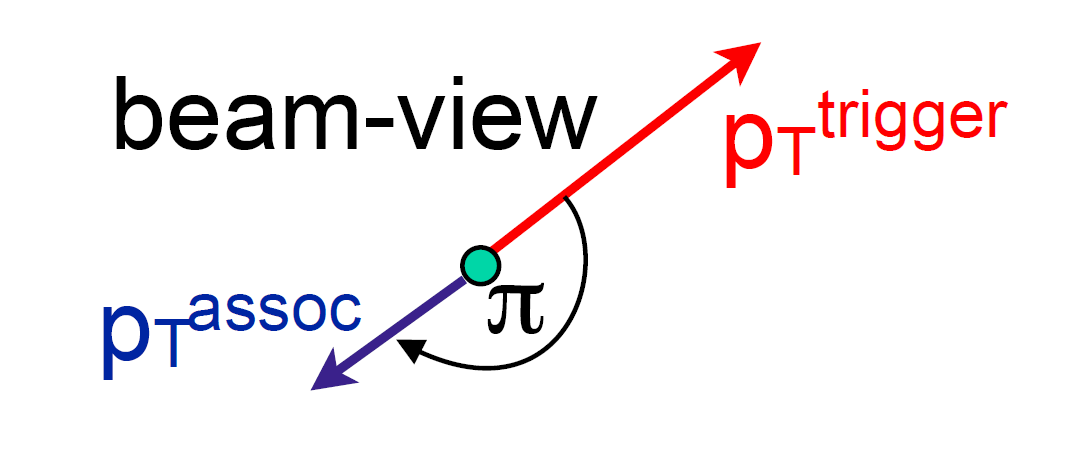
\includegraphics[width=0.4\textwidth]{plots/chpt3/dihadron_beam_view.png}
\caption[A schematic view of the trigger/associate particles in the correlated hadron pairs in the plane perpendicular to the beam direction]{
A schematic view of the trigger/associate particles in the correlated hadron pairs in the plane perpendicular to the beam direction.
This plot is from Ref.~\cite{Accardi:2012qut}.}
\label{fig:dihadron_beamView}
\end{figure}

At sufficiently high parton densities, when
saturation effects dominate, incoming gluons normally carry a typical transverse
momentum at a scale of $Q_{s}>Q$, which significantly increases the transverse
momentum imbalance of the back-to-back jets. As a result, saturated gluons from
the target tend to smear the back-to-back picture and suppress the away-side
peak in the $\Delta\phi$ distribution.

The observed suppressions in dihadron correlation measurements at forward
rapidities performed in \dA\ $\sqrt{s}=200$ GeV collisions at
RHIC~\cite{Adare:2011sc,Braidot:2010ig,Li:2012bn} are perhaps the most
suggestive evidence for the onset of the saturation regime in present data, shown
in Fig.~\ref{fig:dihadron_dAu}. Rather significant suppression of the away-side
correlation is observed, when one compares the data for central \dA\ collisions
to peripheral \dA\ collisions at forward rapidities. The qualitative feature of
this suppression was first predicted by Marquet~\cite{Marquet:2007vb} based on
saturation physics/CGC calculations. The strength of back-to-back correlations
and the depletion of the away-side peak measured in these experiments can be
quantitatively described in the saturation
formalism~\cite{Albacete:2010pg,Stasto:2011ru,Lappi:2012nh}. On the other hand,
a non-CGC framework based on the higher-twist calculation with the nuclear shadowing and the
cold nuclear energy loss correction is also found to be able to reproduce the
suppression phenomenon~\cite{Kang:2011bp}. Generally, the strength of suppression
is expected to be stronger with increasing rapidity, increasing collision centrality
and decreasing transverse momentum of the correlated hadron pairs in \dA\ collisions.

\begin{figure}
\centering
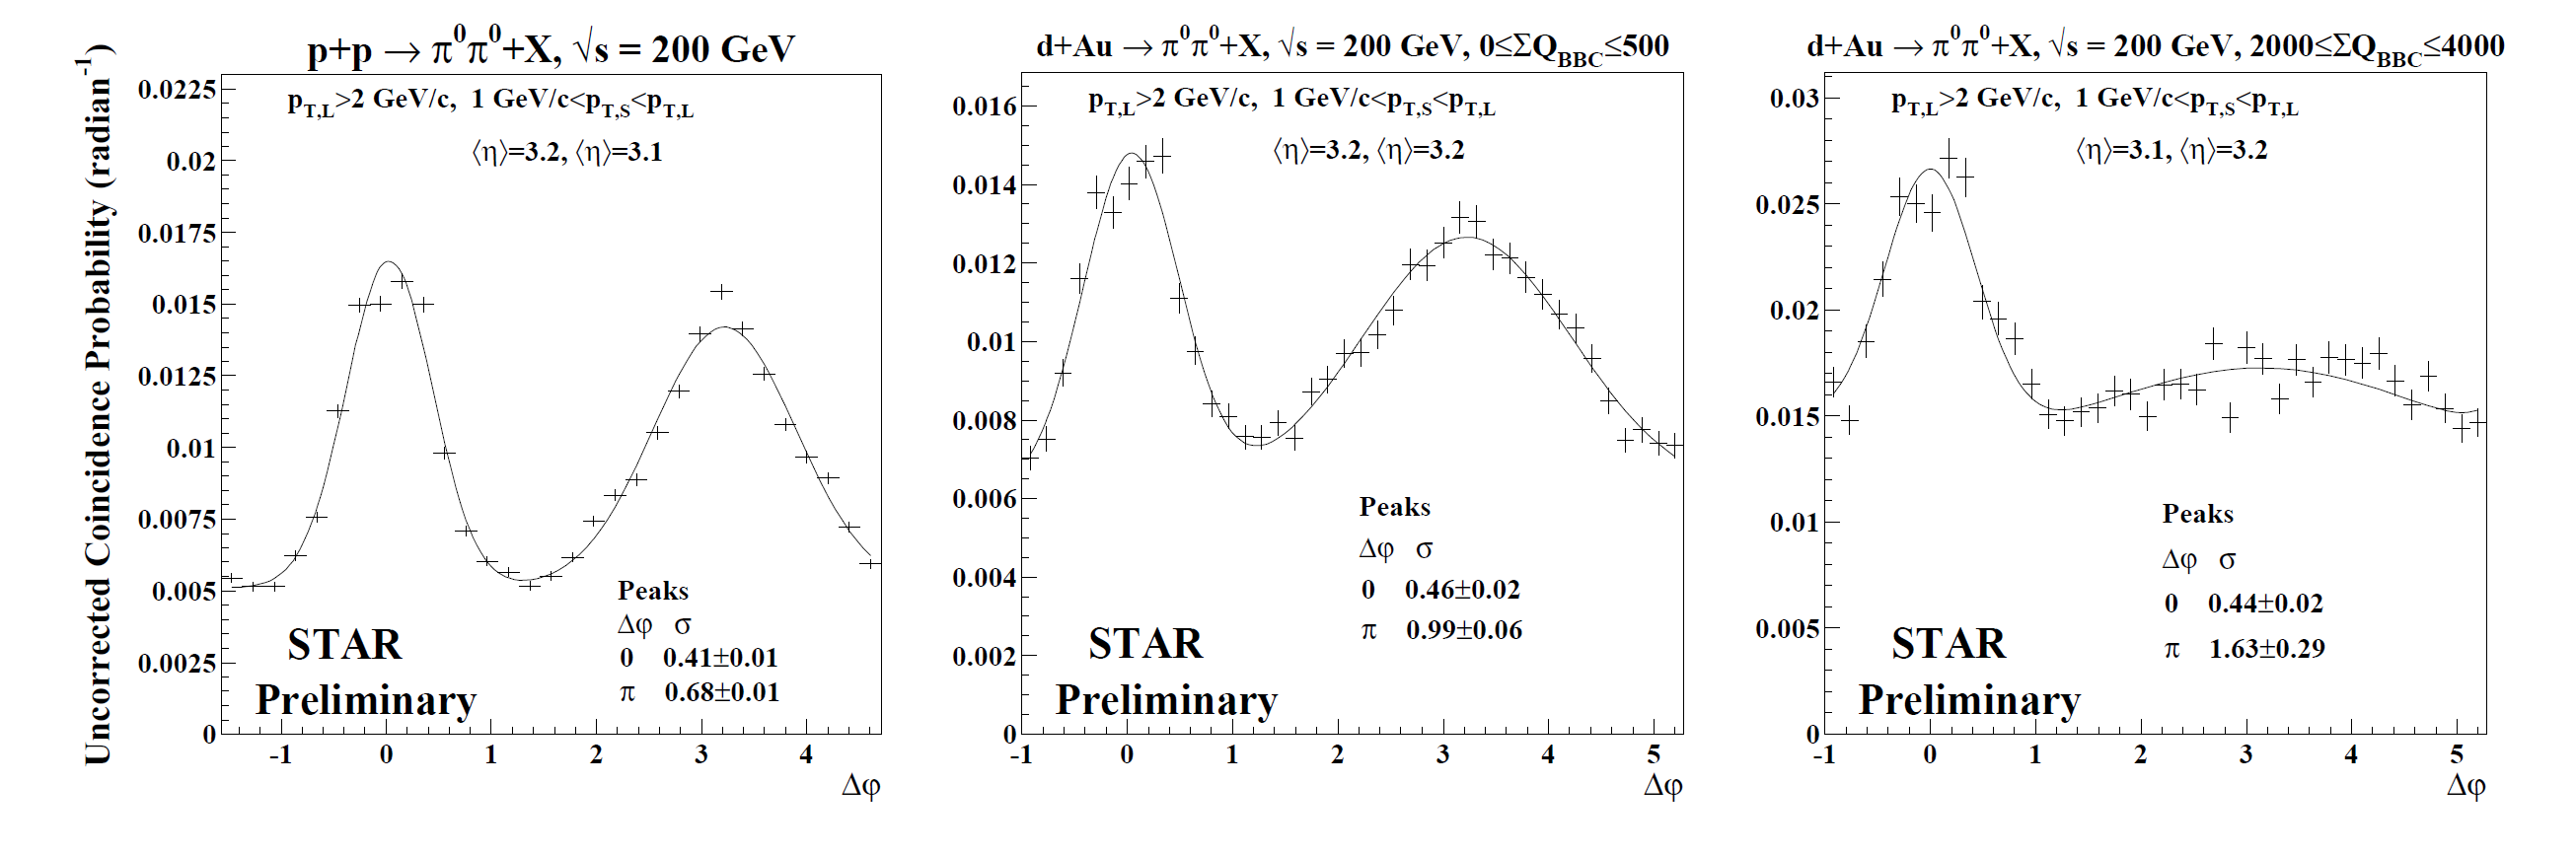
\includegraphics[width=1.0\textwidth]{plots/chpt3/dihadron_pp_dAu_periph_cen.pdf}
\caption[Conditional yield of dihadron correlations in $d+$Au collisions at STAR]{
STAR preliminary results for the two $\pi^{0}$ correlation as a function of the
azimuthal angle difference in $p+p$ and \dA\ ollisions at RHIC. The correlation
function from peripheral and central \dA\ collisions are shown in the middle panel and right
panel respectively.
This plot is from Ref.~\cite{Braidot:2010ig}.}
\label{fig:dihadron_dAu}
\end{figure}

Up to now, it is not possible to extract any definitive conclusion from the
analysis of presently available data. The model dependent kinematics control
introduces a large uncertainty to the data analysis which blurs the
physical interpretation to the phenomenon. Also, the technical difficulty of
higher-order calculations in the CGC also prevents us from achieving a
description of the data precise enough to distinguish different scenarios.
Considering these difficulties, it will be very beneficial to perform the
dihadron correlation study in the \eA\ collisions at an EIC with much better
kinematics control and much less final state contaminations. Besides,
considering it is a single unintegrated gluon distribution structure involved in
\eA\ dihadron correlations instead of a mixture of two types of gluon distribution
involved in \dA\ , the information extracted from the \eA\ dihadron studies will
be complementary to the understanding of phenomenon observed in \dA\ .



At an EIC, we can access dihadron correlations in deep inelastic scattering
(DIS) data from \eA\ and \ep\ collisions, which can provide a clean and
well-controlled signature of saturation physics complementary to the current \dA\
or \pA\ measurements. They also provide the opportunity to study a fundamental
gluon distribution that cannot be accessed today. It has been shown in the
recent theoretical development of small $x$ physics that there are two different
unintegrated gluon distributions (UGDs); namely the Weizs\"{a}cker-Williams (WW)
gluon distribution and the dipole gluon distribution, which are involved in the
calculation of various observables~\cite{Dominguez:2010xd}. Since all other
gluon distributions appearing in various processes can be constructed from these
two UGDs in the large $N_c$ limit of QCD, they can be considered as the
universal and fundamental building blocks for all UGDs. Furthermore, the WW
gluon distribution can be interpreted as the gluon density in the light cone
gauge, while the dipole gluon distribution has no such probabilistic
interpretation. In addition, we want to emphasize that the WW gluon distribution
appears in few physical processes exclusively, and currently there is very
little knowledge about its behavior. Fortunately, the WW gluon distribution is
the only UGD involved in the DIS dijet process~\cite{Dominguez:2011wm}, which
provides us a unique and clean means to measure the WW gluon distribution.



